\documentclass[.../bericht]{subfilies}

\begin{document}

  \section{Introduction}

    This experiments serves to examine the position fluctuations of polystyrene particles with a diameter of
    \begin{equation*}
      a=\SI{4,28}{\micro\meter}
    \end{equation*}
    in an aqueous dispersion that is highly dilute. The observed motion is called the \textit{Brownian motion} (compare \cref{sec:brownian-motion}). To this end, the form of the potential surrounding the single particles is to be determined. Moreover, the determination of the dependency of the diffusion coefficient on the distance between particle and the walls of the cuvette containing the dispersion along with the total distance for a given particle are main goals of the experiment. Regarding the used optical tweezers, the light force on the particles is measured. Last, through measurements of silica particles' movement in aqueous dispersions with different concentrations of salt, the variation of the screening length is examined.


    \section{Brownian motion}
    \label{sec:brownian-motion}

      The motion of particles suspended in a fluid resulting from their collision with fast moving molecules (or atoms) of the fluid is called the \textit{Brownian motion}.

      Within a fluid at thermal equilibrium at a given temperature, no preferential direction of flow exists. Therefore, the movement the fluid's molecules is random yielding no linear or angular momenta over time. Suffieciently small particles suspended in this fluid move in random patterns, too, changing its velocity $\vec{v}$ upon colliding with one of the fluid's molecules. As a matter of fact, the observation has been used as evidence for the existence of individual water (fluid) molecules.

      Because of the sheer number of involved fluid molecules, the many-body interactions resulting in the \textit{Brownian motion} cannot be solved relying only on classical mechanics. To put a number to it, the number of collisions of a single particle suspended in the fluid (a so called \textit{Brownian particels}) with the fluid molecules is roughly of the order $10^{14}$. Therefore, among other, Albert Einstein produced a probabilistic model using statistical mechanics. Einstein started by formulating a diffusion equation for the \textit{Brownian particels}. To this end, he regarded a one dimensional $x$-space with the origin at the initial position of the modelled \textit{Brownian particles}. Assuming the conservation of the number of fluid molecules and introducing the density function $\varphi(\Delta)$, with the random variable $\Delta$, he expanded the \textit{Brownian particle} density $\rho$ at a time $t + \tau$ in a Taylor series
      \begin{align*}
        \rho (x,t) + \tau \pdv{\rho (x)}{t}+\cdots=\rho (x,t+\tau )&= \rho (x,t)\cdot \int_{-\infty}^{\infty} \varphi (\Delta )\mathrm{d}\Delta \\
        &=\rho(x,t)\cdot\int_{-\infty}^{\infty} \varphi (\Delta ) \mathrm{d}\Delta  -\pdv{\rho}{ x}\cdot \int_{-\infty}^\infty \Delta \varphi (\Delta )\mathrm{d} \Delta \\
        &\quad + \pdv[2]{\rho}{x}\cdot \int_{-\infty}^{\infty} \frac{\Delta^2}{2} \varphi (\Delta ) \mathrm{d} \Delta + \cdots \\
        &=\rho(x,t)\cdot 1 +0+\pdv[2]{\rho}{x}\cdot \int_{-\infty}^{\infty} \frac{\Delta^2}{2}\varphi(\Delta ) \mathrm{d}\Delta +\cdots.
      \end{align*}
      While the integral in the second line equals one by definition of the probability, terms with even partials vanish due to symmetry of the 1D space. The above equation is equivalent to
      \begin{align}
        \pdv{\rho}{t}&\approx\pdv[2]{\rho}{x}\cdot \int_{-\infty}^{\infty} \frac{\Delta^2}{2\tau} \varphi ( \Delta) \mathrm{d}\Delta \nonumber  \\
        &=D\cdot \pdv[2]{\rho}{x}  \label{eq:diffusion-equation}
      \end{align}
      if only terms with orders smaller than 2 of $\Delta$ are regarded and using the \textit{mass diffusivity} or \textit{diffusion coefficient}
      \begin{equation}
        D=\int_{-\infty}^{\infty} \frac{\Delta^2}{2\tau} \varphi ( \Delta) \mathrm{d}\Delta.
        \label{eq:diffusion-coefficient}
      \end{equation}


      \subsection{Brownian motion in proximity of the cavity walls}
      \label{subsec:brownian-wall}

        In \cref{sec:brownian-motion}, only the fluid's molecules surrounding the \textit{Brownian particles} have been taken into account for the diffusion equation \cref{eq:diffusion-equation}. When the fluid is confined in a cavity though, the cavity's walls affects the flow of the fluid. This statement can be proven by simply regarding a fluid molecule or \textit{Brownian particle} next the cavity wall. It's motion'S component orthogonal to the wall is limited to one direction which is away from the wall. The interaction between the confining walls andthe particles is called \textit{hydrodynamic interaction}.

        The mathematical description of this phenomenon makes use of distance $z$ dependent diffusion coefficients
        \begin{align}
          D_\parallel(z)&=D_0\left[ 1- \frac{9}{16} \left( \frac{a}{z+a}\right) + \frac{1}{8} \left( \frac{a}{z+a}\right)^3 - \frac{45}{256}\left( \frac{a}{z+a}\right)^4- \frac{1}{16}\left( \frac{a}{z+a}\right)^5+\cdots \right] \label{eq:D-parallel} \\
          D_\perp(z)&=D_0\left[ \frac{4}{3}\sinh (\alpha ) \sum_{n=0}^{\infty} \frac{n(n+1)}{(2n-1)(2n+3)}\left( \frac{2\sinh ((2n+1)\alpha )+(2n+1)\sinh (2\alpha )}{4\sinh^2 ((n+ \frac{1}{2})\alpha)-(2n+1)^2 \sinh^2 (\alpha )} - 1 \right) \right]^{-1} \nonumber \\
          &\approx D_0\cdot \frac{6 \left( \frac{z}{a}\right)^2 + 2 \frac{z}{a}}{6\left( \frac{z}{a}\right)^2 + 9 \frac{z}{a} + 2} \label{eq:D-perp}
        \end{align}
         for the motion orthogonal ($\perp$) and parallel ($\parallel$) to the walls, where $z$ is the distance between particle and wall and $\alpha=\arccos \left( \frac{z+a}{a} \right)$. For the approximation of \cref{eq:D-perp} please refer to \cite{beavan}. The diffusion coefficients are plotted in \cref{fig:D-wall}. As expected from the thought experiment this section has been introduced with, $D_\perp (z=0)=0$, whereas $D_\parallel (z=0)\ne 0$. \cite{helden}

         \begin{figure}
           \centering
           \tikzsetnextfilename{D_walls}
           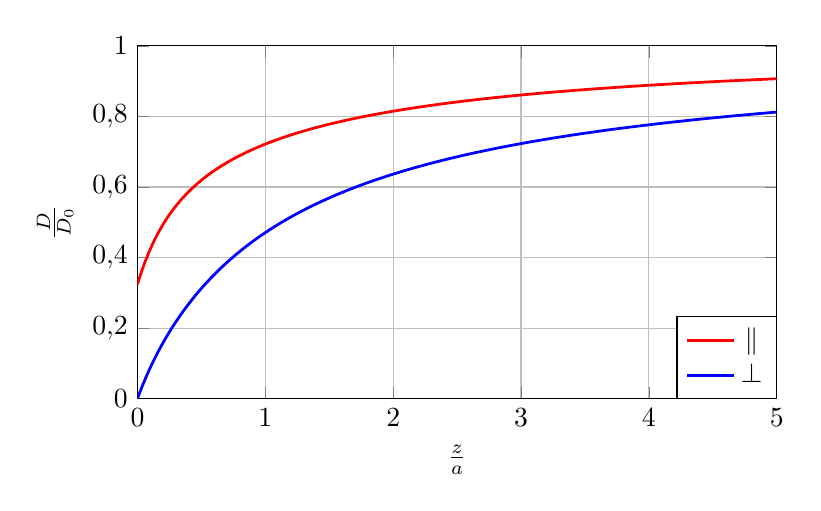
\begin{tikzpicture}
               \begin{axis}[
                 /tikz/line join=bevel,
                 width=0.8*\textwidth,
                 height=0.5*\textwidth,
                 grid,
                 legend style={at={(1,0)}, legend columns=1, anchor=south east},
                 every axis plot,
                 xmin = 0, xmax = 5,
                 ymin = 0, ymax = 1,
                 ylabel = {$\frac{D}{D_0}$},
                 xlabel = {$\frac{z}{a}$},
                 /pgf/number format/use comma,
                 /pgf/number format/1000 sep={},
                 ]
                 % Add plots
                 \addplot[domain=0.00001:5,samples=500, unbounded coords=discard, color=red, line width=1pt] {1-9/16*(x/(x^2+x))+1/8*(x/(x^2+x))^3-45/256*(x/(x^2+x))^4-1/16*(x/(x^2+x))^5};
                 \addlegendentry{$\parallel$}
                 \addplot[domain=0:5,samples=500, unbounded coords=discard, color=blue, line width=1pt] {(6*x^2+2*x)/(6*x^2+9*x+2)};
                 \addlegendentry{$\perp$}
               \end{axis}
           \end{tikzpicture}
           \caption{Distance dependent diffusion coefficients for a particle of diameter $a$ at a distance $z$ from the walls for parallel and perpendicular components of motion (compare \cref{subsec:brownian-wall}).}
           \label{fig:D-wall}
         \end{figure}


      \section{Forces on the Particles}
      \label{sec:forces}

        There are several forces affecting particles suspended in a solution. Most relevant for this experiment are the gravitational force, the electrostatic double layer force, the Van der Waals force and the light force (when using the optical tweezers).
        \textbf{Gravitational force:}\\
        The particles interact with the gravitational field of the earth. If their density is higher then the density of the solution they are suspended in they sink to the bottom. In front of a wall were it is affected by a repulsive force a potential well forms.  The gravitational potential $V_\mathrm{G}$ can be described as:
        \begin{align}
          V_\mathrm{G}=\frac{4\pi R^3}{3}g(\rho_p-\rho_m)z=F_\mathrm{G}z
        \end{align}
        with the density $\rho$ of the particle (p) and the medium (m), the earth acceleration $g$, the particles radius $R$ and the distance from the wall $z$.
        \textbf{Eletrostatic double layer force:}\\
        The eletrostatic double layer force is the repulsion between particles with the same charge and between particles and the wall. If the particles are suspended in an electrolyte solution, as it is the case here, the Poisson equation describes the relation between the electrostatic potential $\Phi (\overrightarrow{r})$ and the elementary charge $e$.
        \begin{align}
          \Delta \Phi (\overrightarrow{r})=-\frac{e^2}{\epsilon k_B T}\rho(\overrightarrow{r})
        \end{align}
        With $e\rho(\overrightarrow{r})=e(\rho_+(\overrightarrow{r})+\rho_-(\overrightarrow{r}))$ with the Kation concentration ($\rho_+(\overrightarrow{r}$) and the Anion concentration ($\rho_-(\overrightarrow{r}$). If the two concentrations are symmetrical as it is the case for monovalent electrolytes (like K Br) the Poisson-Boltzmann-equation is
        \begin{align}
          \Delta \Phi= \kappa^2sinh\Phi,
        \end{align}
        with $\kappa=\sqrt{\frac{\beta e^2}{\epsilon}2\rho_+}=\sqrt{\frac{e^2}{\epsilon k_B T}\sum_i \rho_i z_i^2}$ as the inverse Debye length, with $z_i$ as the ion charge and $r\in G$, with $G$ as the area which is not particle or surface. With the surface-charge-density for particles $\sigma_p$ and wall $\sigma_w$ and $z$ as the distance between particle surface and wall we get
        \begin{align}
          \beta V_{dl}(z)=\frac{64\pi \epsilon a}{\beta e^2} \gamma_p \gamma_w e^{-\kappa(z)} \\
          \gamma_{w/p}=tanh[\frac{1}{2}\sinh^{-1} \left(\frac{\beta e \sigma_{w/p}}{2\epsilon \kappa}\right).
        \end{align}
        \textbf{Van der Waals force:}\\
        In comparison to the previously described electrostatic force the Van der Waals force is much weaker. It is also mostly attractive in nature. Microscopically it stems from the interactions between the fluctuating dipolmoments of the particles. Integration of the particle-particle and the particle-wall Van der Waals force over the sphere wall symmetry of this experiment provides
        \begin{align}
          \beta V_{disp}(z)=\frac{A(z)}{6k_B T}(\frac{2R}{z}\frac{z+R}{z+2R}-log\frac{z+2R}{z}),
        \end{align}
        with the distance between particle surface and wall $z$, $R$ the particle radius and $A(z)$ as the Hamakerconstant.
        \textbf{Light force with optical tweezers:}\\
        To counteract some of the previously mentioned forces optical tweezers can be used to hold particles in place, by utilizing the light force. The light force is the impulses of photons that are transferred to the particle when it absorbs or reflects the photons.
        The simplest case is if the light force or any other one directional force. For gravitation the light beam shines from below with the light force $L_{light}=L_{grav}$. But optical tweezers/traps can also hold dielectric particles in place against forces perpendicular to the light beam. For this a slightly focused laser beam is utilized and the particle is held in the focus point. This is shown in \ref{fig:tweezer}.

        \begin{figure}[tb]
          \centering
          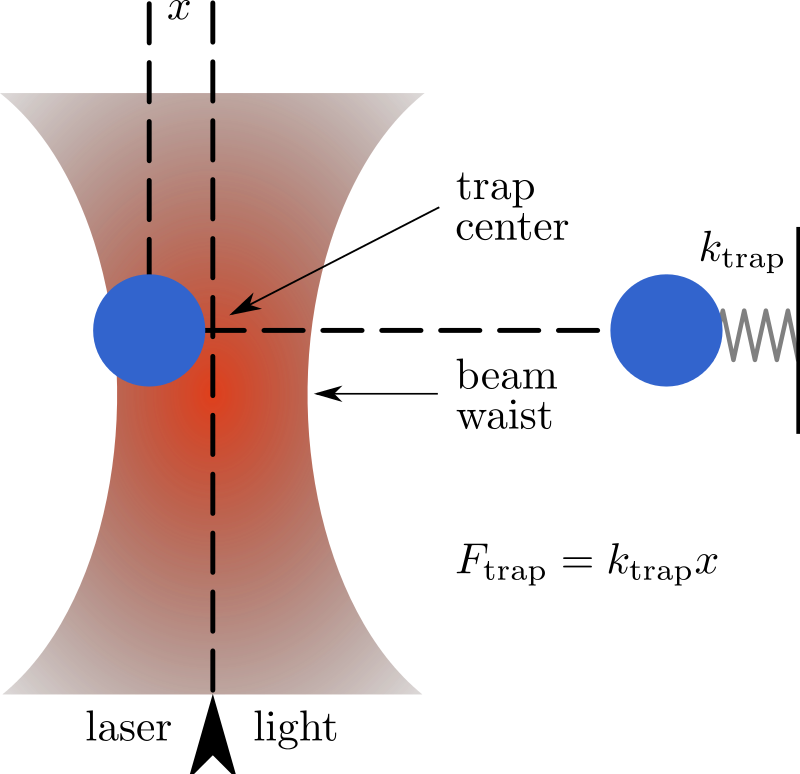
\includegraphics[width=0.5\textwidth]{figures/opticaltweezer}
          \caption{Particle in an optical trap. The dielectric particle gravitates towards the beam center slightly above the beam waist.  %https://en.wikipedia.org/wiki/Optical_tweezers
           }
           \label{fig:tweezer}
        \end{figure}
        The force which moves the particle towards the beam center is called the gradient force. But it only moves the particle towards the center, if the refractive index of the particle is larger then the one of the solution in which it is held. Because, if this is the case and there is and intensity gradient, the gradient force moves the particle towards the point of the highest intensity. Similar to a dielectric being sucked into a capacitor. With a strong focus point it is also possible of the gradient force to override the light force. For optical tweezers in $x$- and $y$-direction the potentials are:
        \begin{align}
          V_{grad,x}(x)=C_xPx^2\\
          V_{grad,y}(y)=C_yPy^2
        \end{align}
        with the laser power $P$ and the parameter $C$ depending on particle size, focus radius, refractive indexes and more. \\
        Finally, for the $z$ direction the light force and the gravitational force add up to
        \begin{align}
          V_{Geff}=V_{Light}+V_{G}=F_{Light}+F_{G} z= G_{eff} z.
        \end{align}




      \section{Evanescent Field}
      \label{sec:evanenscent}

      \section{Determination of the potential form}
      \label{sec:determination}

      \section{Hydrodynamic evaluation}
      \label{sec:hydrodynamic}










\end{document}
